\documentclass[10pt, aspectratio=169]{beamer}

% --- Load Metropolis Theme ---
\usetheme{metropolis} 

% --- Custom Blue Palette Configuration ---
\definecolor{DarkBlue}{RGB}{0, 33, 71}      % Deep Oxford Blue
\definecolor{MidBlue}{RGB}{0, 82, 155}       % Professional Medium Blue
\definecolor{LightBlue}{RGB}{173, 216, 230} % Soft Accent Blue

% Apply colors to Metropolis elements
\setbeamercolor{normal text}{fg=black, bg=white}
\setbeamercolor{alerted text}{fg=MidBlue}
\setbeamercolor{example text}{fg=DarkBlue}

% Customizing the Progress Bar and Frame Titles
\setbeamercolor{palette primary}{bg=DarkBlue, fg=white}
\setbeamercolor{progress bar}{fg=MidBlue, bg=LightBlue}
\setbeamercolor{title separator}{fg=MidBlue}
\setbeamercolor{frametitle}{bg=DarkBlue, fg=white}

% --- Packages ---
\usepackage[utf8]{inputenc}
\usepackage[T1]{fontenc}
\usepackage{amsmath, amsfonts, amssymb, bm}
\usepackage{graphicx}
\usepackage{booktabs}

% --- Title ---
\title{Copula Markov Chains for Dependent Extremes}

\setbeamertemplate{title page}{
  \centering

  {\usebeamerfont{title}\inserttitle\par}
	\vspace{-0.5em}

	\textcolor{DarkBlue}{\rule{\textwidth}{0.5pt}}
	
  {\usebeamerfont{author}\insertauthor\par}
  \vspace{0.3cm}

  {\usebeamerfont{institute}\insertinstitute\par}
  \vspace{0.3cm}

  {\usebeamerfont{date}\insertdate\par}

  \vfill

  % logos at bottom
  
\includegraphics[height=1cm]{logo_um.png}
  \hspace{0.5cm}
  
\includegraphics[height=1.2cm]{logo_imag.png}
	\hspace{0.5cm}
	
\includegraphics[height=1cm]{inr_logo_grisbleu.png}
  \vspace{0.5cm}
}

\author{
  \textbf{Andrea Ferrero}$^{1}$\\[0.2cm]
  \small Supervised by: Gwladys Toulemonde$^{1}$, Nicolas Meyer$^{1}$, Klaus Herrmann$^{2}$
}

\institute{
  $^{1}$ \textit{University of Montpellier, Lemon Team Inria} \\
  $^{2}$ \textit{University of Sherbrooke}
}

\date{}

\titlegraphic{
  
\includegraphics[height=1cm]{logo_um.png}
  \hspace{0.5cm}
  
\includegraphics[height=1cm]{logo_imag.png}
}

\begin{document}

\maketitle

% ==========================================
% SECTION 1: FOUNDATIONS
% ==========================================
\section{Foundations}

\begin{frame}{GEV: The Limit Distribution of Maxima}

  \begin{block}<1->{}
    Assume $X_1, \dots, X_n$ are \alert{i.i.d.} random variables from a distribution $F$. Let $M_n = \max(X_1, \dots, X_n)$. 
  
    If there exist sequences $a_n > 0$ and $b_n$ such that:
    \[
    P\left( \frac{M_n - b_n}{a_n} \le x \right) \xrightarrow{n \to \infty} G_\xi(x)
    \]
    then $G_\xi$ is a \alert{Generalized Extreme Value (GEV)} distribution. We say that $F$ is in the \textbf{maximum domain of attraction} (MDA) of $G_\xi$.
  \end{block}

  \begin{block}<2->{}
  The \textbf{shape parameter} $\xi$ (tail index) defines the margin tail behavior:
  
  \begin{itemize}
    \item \textbf{$\xi > 0$:} \textbf{Fréchet} (Heavy-tailed, e.g., Pareto, Cauchy)
    \item \textbf{$\xi = 0$:} \textbf{Gumbel} (Exponential-like, e.g., Normal, Gamma)
    \item \textbf{$\xi < 0$:} \textbf{Weibull} (Bounded upper tail, e.g., Uniform, Beta)
  \end{itemize}
  \end{block}
  
\end{frame}

\begin{frame}{GPD: The Limit Distribution of Exceedances}
    For a sufficiently high threshold $u$, we consider the distribution of the \alert{exceedances} $Y = X - u$, given that $X > u$. If $F \in MDA(G_\xi)$, with $G_\xi$ a GEV distribution, then:
    
    
    \[
    P(X - u \le y \mid X > u) \xrightarrow{u \to \infty} H_{\xi, \sigma}(y) = \begin{cases}
		1 - \left( 1 + \xi \frac{y}{\sigma} \right)^{-1/\xi}, & \xi \neq 0, y > 0 \\
		1 - \exp\left( -\frac{y}{\sigma} \right), & \xi = 0, y > 0
		\end{cases}
    \]
   
		where $H_{\xi, \sigma}$ is the \alert{Generalized Pareto Distribution (GPD)}

\end{frame}

\begin{frame}{Modelling Block Maxima with GEV}
	\begin{figure}
		\centering
		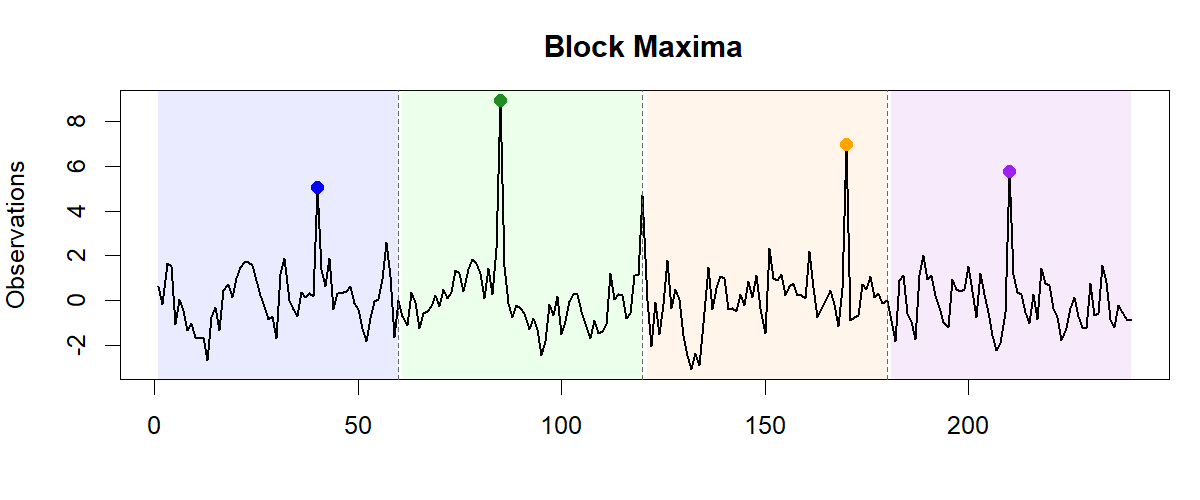
\includegraphics[width=\textwidth]{figures/block_maxima.png}
	\end{figure}
\end{frame}

\begin{frame}{POT: Modelling Exceedances with GPD}
	\begin{figure}
		\centering
		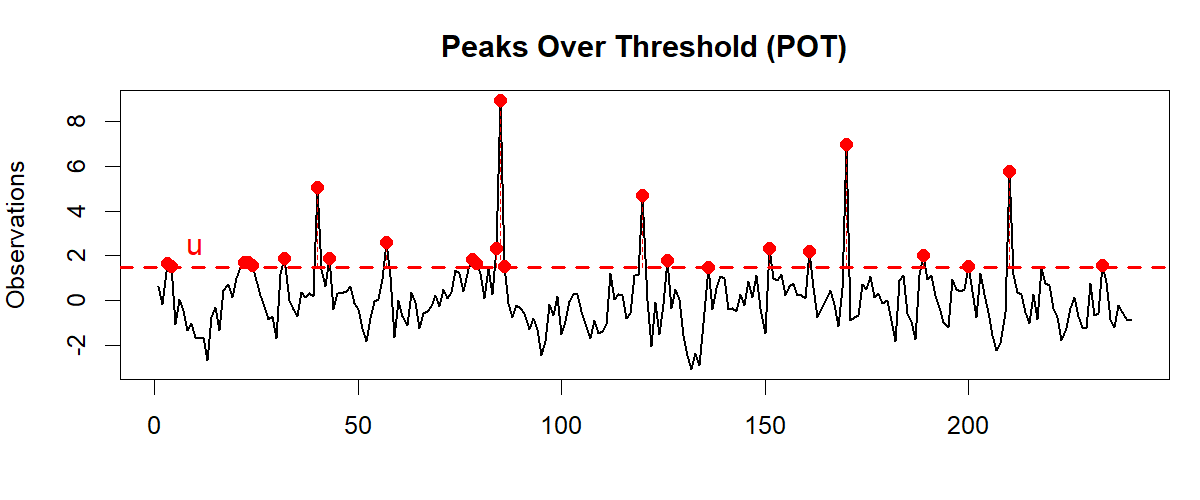
\includegraphics[width=\textwidth]{figures/pot_threshold.png}
	\end{figure}
\end{frame}

\begin{frame}{Threshold Stability Plot: Choosing the Threshold}
	\begin{figure}
		\centering
		
\includegraphics[width=\textwidth]{figures/gpd_threshold_stability.png}
	\end{figure}
\end{frame}

\begin{frame}{Hill Estimator: a semi-parametric approach for $\xi > 0$}
    Assume $F$ has a regularly varying tail: $\bar{F}(x) = x^{-1/\xi} L(x)$, with $\xi > 0$ and $L(x)$ a slowly varying function. \pause

    Given the order statistics $X_{(1)} \ge X_{(2)} \ge \dots \ge X_{(n)}$, the Hill estimator is defined as:
    \[
    \hat{\xi}_H(k) = \frac{1}{k} \sum_{i=1}^{k} \log \left( \frac{X_{(i)}}{X_{(k+1)}} \right)
    \]
		
\end{frame}

\begin{frame}{Hill Plot: Choosing the Number of Order Statistics}
	\begin{figure}
		\centering
		
\includegraphics[width=\textwidth]{figures/hill_plot.png}
	\end{figure}
\end{frame}


 \begin{frame}{Asymptotic Normality of Hill Estimator}
    Under certain (second order) conditions on the tail of the distribution, Hill's estimator is asymptotically normal but biased:

        \[
        \sqrt{k} \left( \hat{\xi}_H - \xi \right) \xrightarrow{d} N\left( \frac{\lambda}{1-\rho}, \frac{1}{\xi^2} \right)
        \] with $\rho \leq 0$ and $\lambda$ a finite constant.
        \pause

    \begin{itemize}
        \item \textbf{Bias Correction:} Requires estimating $\rho$.
        \item \textbf{Dependence:} \cite{dehaan2016} shows correction under \alert{$\beta$-mixing}
    \end{itemize}
\end{frame}

% \begin{frame}{Generalized Hill Estimator ($\xi \in \mathbb{R}$)}

%     \begin{itemize}
%         \item \textbf{Local Hill Statistic:} $H_{j,n} = \frac{1}{j} \sum_{i=1}^{j} \log X_{(i)} - \log X_{(j+1)}$ \pause
%         \item \textbf{Empirical Substitute ($UH$):} Under general MDA, the quantity $UH = X_{(j+1)} H_{j,n}$ is regularly varying with index $\xi$. \pause
%     \end{itemize}

%     \begin{block}{The Estimator}
%         Estimated as the slope of the generalized quantile plot:
%         \[
%         \hat{\xi}^H_{k,n} = \frac{1}{k} \sum_{j=1}^{k} \log UH_{j,n} - \log UH_{k+1,n}
%         \]
%     \end{block}

% \end{frame}

\begin{frame}{Extended GPD: Avoiding Threshold Selection}
    The idea is to transform the GPD by a suitable distortion function $G(u)$ \cite{naveau2016}. \pause

    \begin{block}{Power Transformation}
        For a random variable $X > 0$, the EGPD CDF is:
        \[
        F(x) = \left[ H_{\xi, \sigma}(x) \right]^\kappa
        \]
        where $H_{\xi, \sigma}(x)$ is the GPD CDF and \alert{$\kappa > 0$} is a bulk parameter.
    \end{block} \pause

    \textbf{Tail Consistency:} For any $\kappa > 0$, the tail behavior remains governed by $\xi$. The EGPD and GPD share the \alert{same tail index}.
\end{frame}

\begin{frame}{EGPD vs GPD: bulk change}
	\begin{figure}
		\centering
		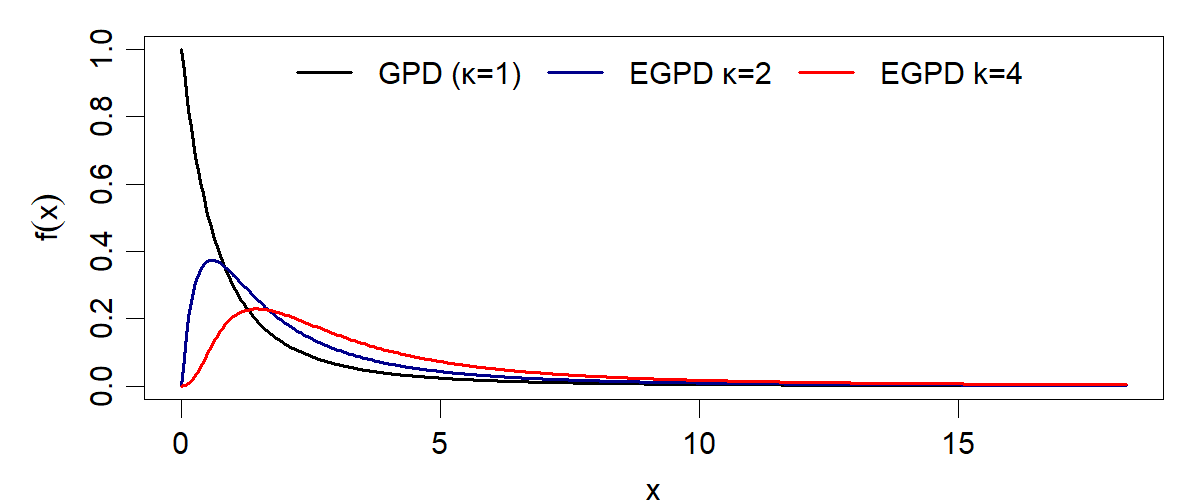
\includegraphics[width=\textwidth]{figures/egpd_plot.png}
	\end{figure}
\end{frame}

\begin{frame}{EGPD vs GPD: tail consistency}
	\begin{figure}
		\centering
		
\includegraphics[width=\textwidth]{figures/egpd_tail_equivalence.png}
	\end{figure}
\end{frame}

% ==========================================
% SECTION 2: DEPENDENCE
% ==========================================
\section{Dependence}

\begin{frame}{Long-Range Dependence: $D(u_n)$ Condition}
    
    \begin{block}{$D(u_n)$ Condition \cite{leadbetter1974}}
        A stationary sequence $\{X_n\}$ satisfies $D(u_n)$ if for any $1 \le i_1 < \dots < i_p < j_1 < \dots < j_q \le n$ with $j_1 - i_p > l$:
        \[ |P(X_{i_1, \dots, i_p} \le u_n, X_{j_1, \dots, j_q} \le u_n) - P(X_{i_1, \dots, i_p} \le u_n)P(X_{j_1, \dots, j_q} \le u_n)| \le \alpha_{n,l} \]
        where $\alpha_{n,l_n} \to 0$ for some $l_n$ s.t. $l_n/n \to 0$ as $n \to \infty$
    \end{block}

    \textbf{Intuition:} Extreme events occurring far apart in time behave as if they were independent.
\end{frame}

\begin{frame}{Distribution of Maxima of Stationary Sequences}

    Assume $\{X_n\} \sim F$ is a stationary sequence satifying $D(u_n)$ with maximum $M_n$. Assume also that for the i.i.d. sequence $\{X^*_n\} \sim F$, the associated maxima $M^*_n$ has GEV limit $G_\xi$. \pause Then, for a constant $0 < \theta \leq 1$,

    \[
    P \left(\frac{M_n - b_n}{a_n} \le x \right) \xrightarrow{n \to \infty} G_\xi^\theta(x).
    \] \pause

    The \alert{extremal index} $\theta$ quantifies the degree of clustering (dependence) of extremes:
    \begin{itemize}
        \item $\theta = 1$: No clustering (i.i.d. case).
        \item $\theta < 1$: Exceedances cluster.
    \end{itemize} \pause

    \textbf{Note:} There exist dependent sequences with $\theta = 1$.
\end{frame}

\begin{frame}{Threshold Exceedances and Declustering}
    Under dependence, exceedances over a threshold $u$ are typically modelled using \alert{declustering}:

    \begin{enumerate}
        \item<1-> Identify \alert{clusters} of extremes (\alert{How?})
        \item<2-> Retain only the \alert{maximum} of each cluster.
        \item<3-> Fit the GPD to these cluster maxima (assumed independent).
    \end{enumerate}

    \vspace{0.3cm}

    \begin{figure}
        \centering

        % Overlay 1
        \only<1>{
            
\includegraphics[width=\textwidth]{figures/declustering1.png}
        }

        % Overlays 2 and 3
        \only<2-3>{
            
\includegraphics[width=\textwidth]{figures/declustering2.png}
        }

    \end{figure}

\end{frame}
% ==========================================
% SECTION 3: COPULA MARKOV MODELS
% ==========================================
\section{Copula Markov Models}

\begin{frame}{Copulas: Decoupling Margins from Dependence}
    A \textbf{Copula} is a multivariate distribution function with uniform marginals on $[0,1]$. \pause

    \begin{block}{Sklar's Theorem (Bivariate Case)}
        For a joint distribution $F_{X,Y}$ with continuous marginals $F_X$ and $F_Y$, there exists a unique copula $C$ such that:
        \[ F_{X,Y}(x,y) = C(F_X(x), F_Y(y)) \] and viceversa.
    \end{block} \pause

    \textbf{Relevance to EVT:}
    \begin{itemize}
        \item We can choose a specialized margin (e.g., \alert{EGPD}) for extremes.
        \item We can choose a copula $C$ that captures \alert{tail dependence} (the probability of co-occurring extremes).
    \end{itemize}
\end{frame}

\begin{frame}{Gumbel Copula}
    \begin{figure}
        \centering
        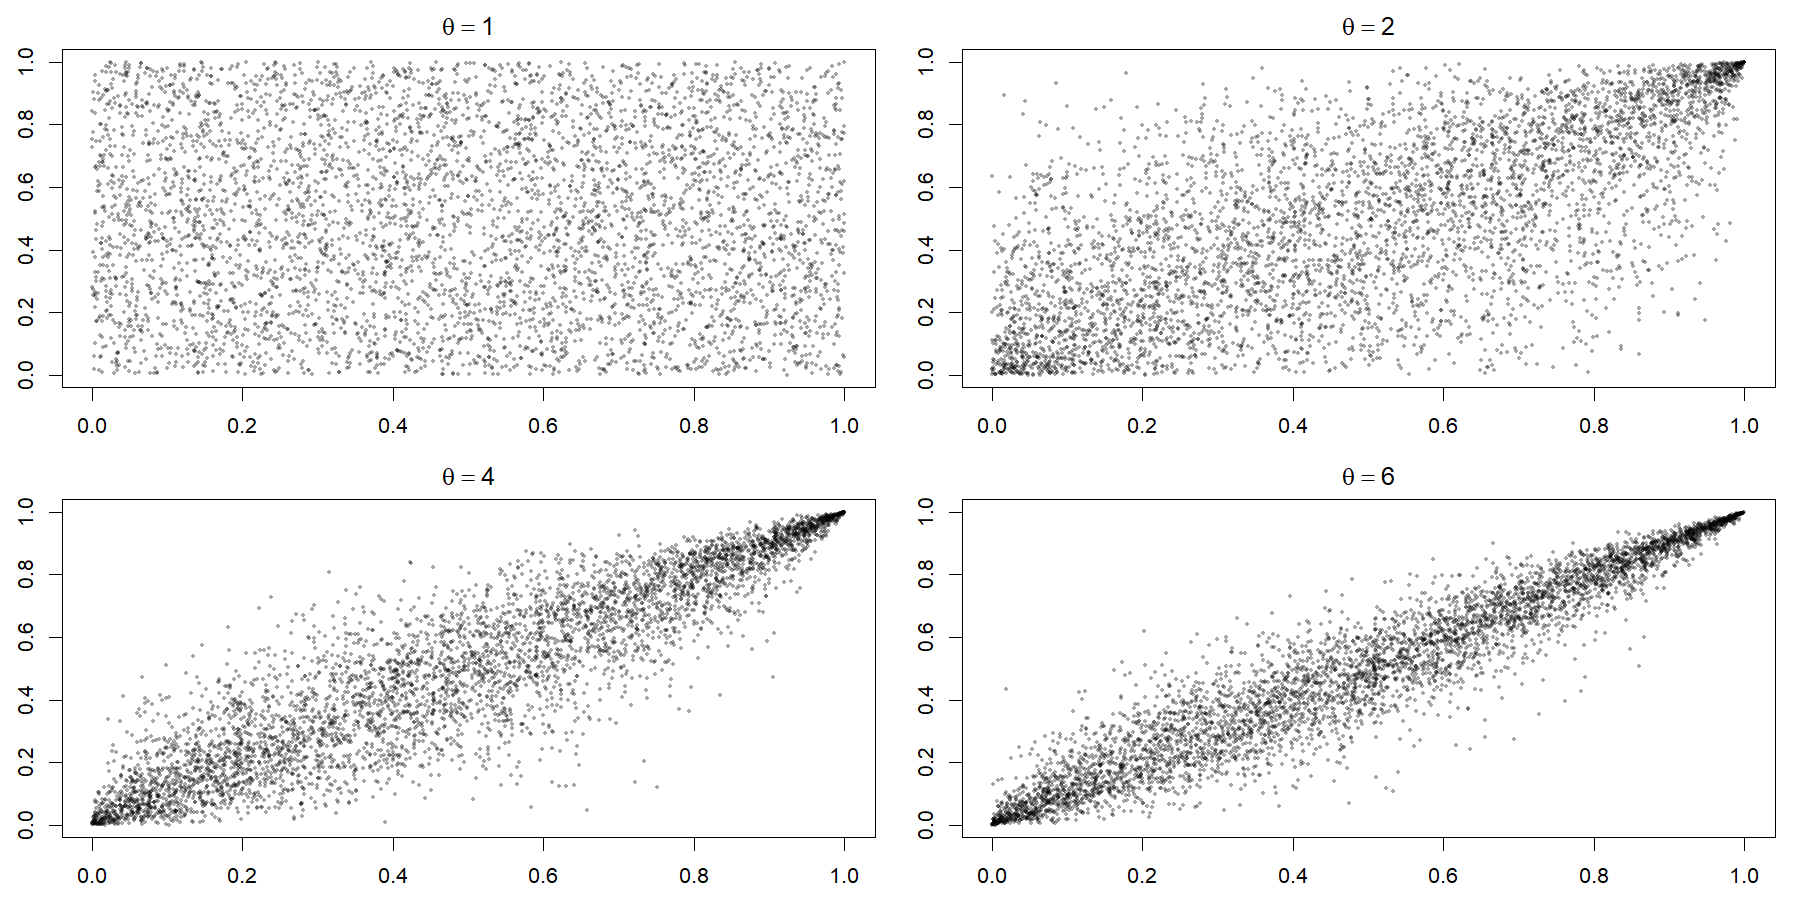
\includegraphics[width=\textwidth]{figures/gumbel_copula.png}
    \end{figure}
\end{frame}

\begin{frame}{Gumbel Copula: Upper Tail}
    \begin{figure}
        \centering
        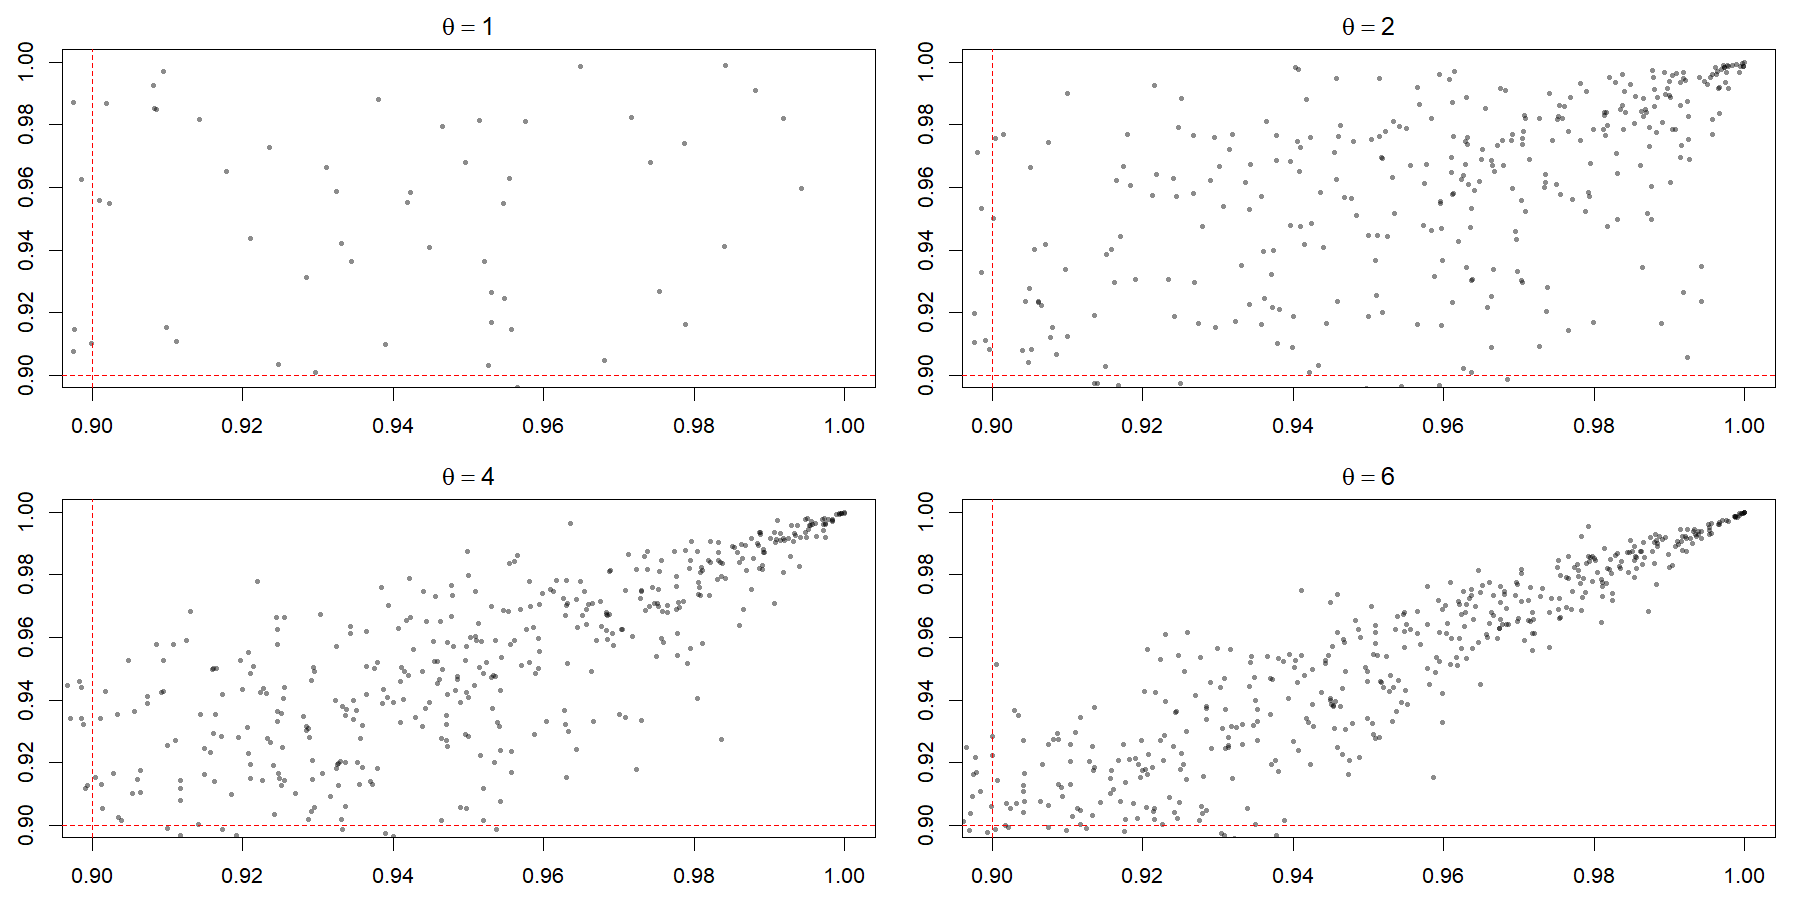
\includegraphics[width=\textwidth]{figures/gumbel_upper_tail.png}
    \end{figure}
\end{frame}

\begin{frame}{Gumbel Copula: Lower Tail}
    \begin{figure}
        \centering
        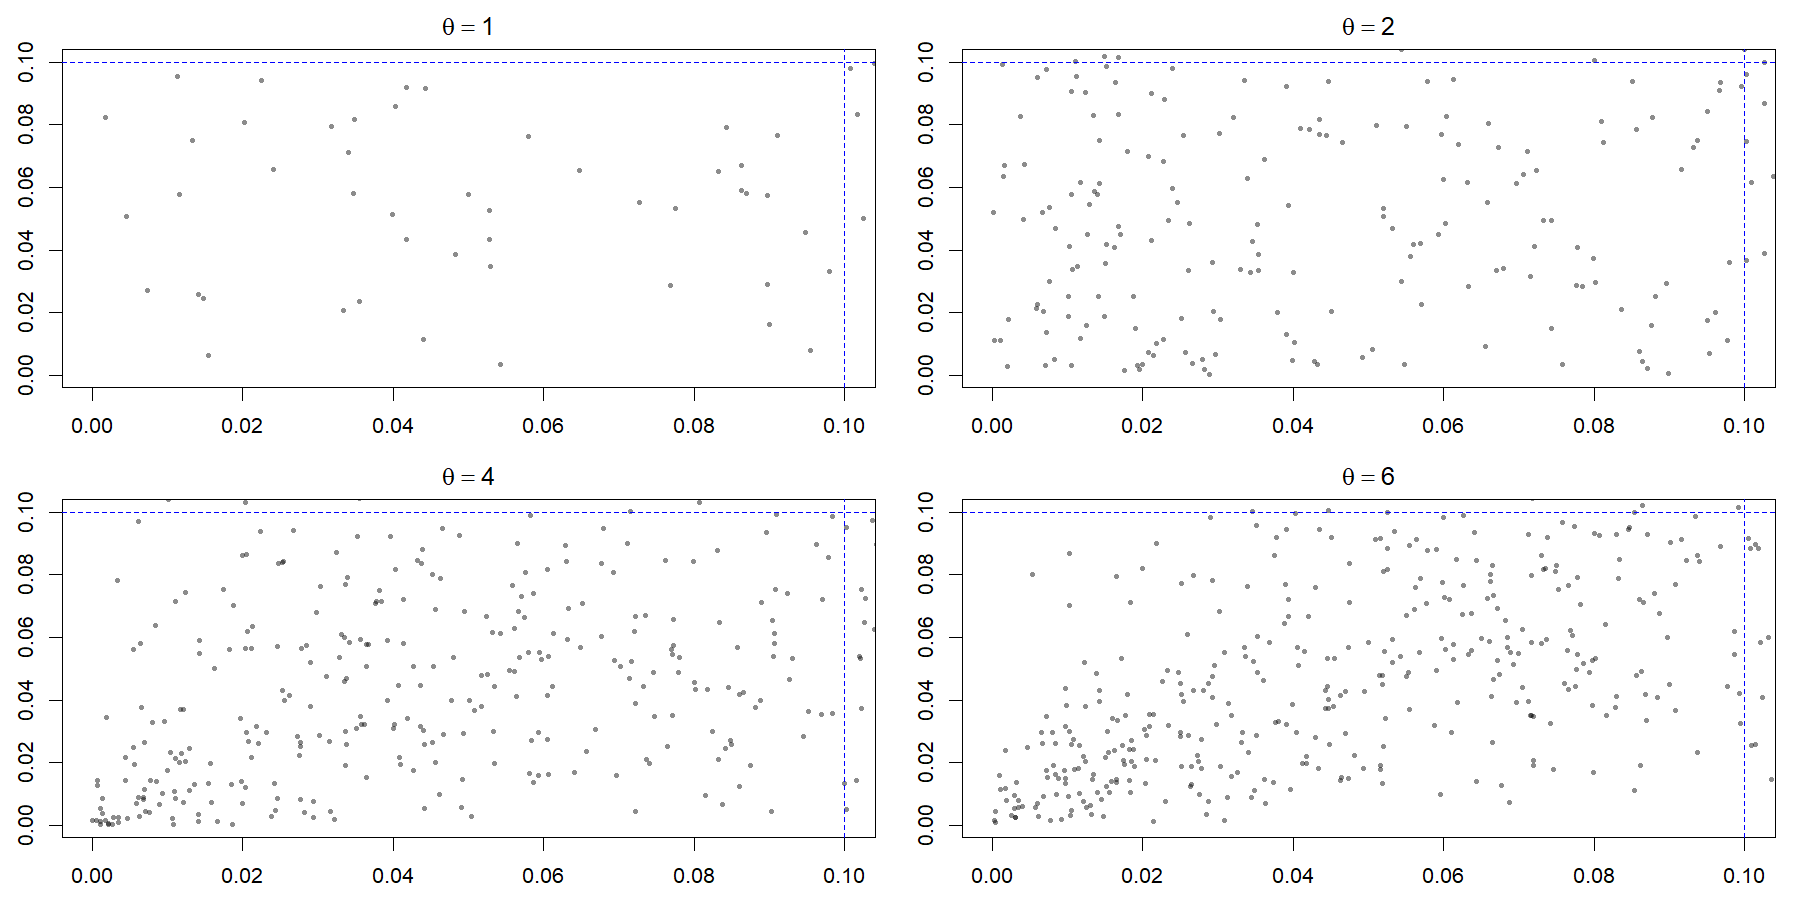
\includegraphics[width=\textwidth]{figures/gumbel_lower_tail.png}
    \end{figure}
\end{frame}

\begin{frame}{Copula Markov Chains}
    
    A stationary first-order Markov chain $\{X_t\}$ is fully defined by its marginal distribution $F$ and the copula $C$ of the pair $(X_{t-1}, X_t)$.

    \begin{overprint}
        \onslide<1>
        \begin{block}{Joint Distribution}
            \[ F_{X_{t-1}, X_t}(x_{t-1}, x_t) = C(F(x_{t-1}), F(x_t)) \]
        \end{block}

        \begin{block}{Conditional Distribution}
            \[ 
            P(X_t \le x_t \mid X_{t-1} = x_{t-1}) = \frac{\partial}{\partial u} C(u, F(x_t)) \Big|_{u=F(x_{t-1})} 
            \]
        \end{block}

        \onslide<2>
        \begin{block}{Sampling}
            \vspace{0.2cm}
            \begin{enumerate}
                \item Sample $U_t \mid U_{t-1}$ s.t. $(U_{t-1}, U_t) \sim C$ (Rosenblatt transform)
                \item $X_t = F^{-1}(U_t)$
            \end{enumerate}
        \end{block}
    \end{overprint}
\end{frame}

\begin{frame}{Simulation Example: EGPD(2,1,0.1) - Gumbel(3)}
    \begin{figure}
        \centering
        
\includegraphics[width=\textwidth]{figures/copula_markov.png}
    \end{figure}
\end{frame}

\begin{frame}{Correlation structure}
    \begin{figure}
        \centering
        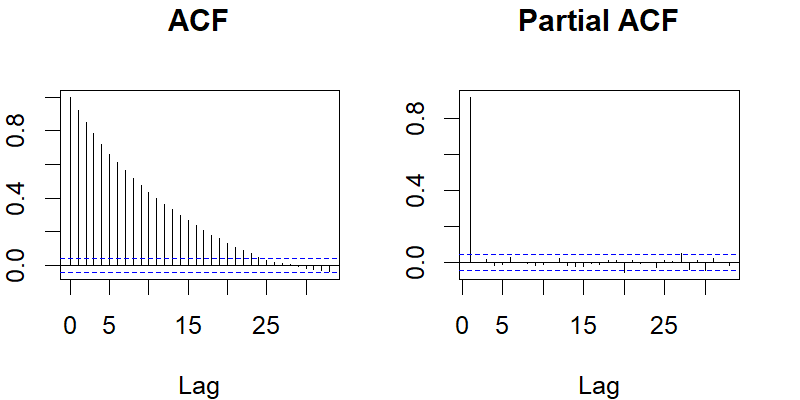
\includegraphics[width=\textwidth]{figures/egpd_gumbel_acf_pacf.png}
    \end{figure}
\end{frame}

\begin{frame}{Inference Strategies for Copula Models}
    Estimating model parameters is usually done via:

    \begin{overprint}
        \onslide<1>
        \begin{block}{1. Inference Functions for Margins (IFM)}
            A two-step estimator:
            \begin{enumerate}
                \item Estimate marginal parameters $\hat{\bm{\theta}}_{m}$ assuming i.i.d. observations.
                \item Estimate copula parameters $\hat{\bm{\theta}}_{c}$ given the fitted margins $\hat{F} = F_{\hat{\theta_m}}$ by maximising copula log-likelihood.
            \end{enumerate}
        \end{block}

        \onslide<2>
        \begin{block}{2. Full Joint Likelihood}
            Simultaneous estimation by maximizing the complete log-likelihood. For a copula markov model:
            \[ \ell(\bm{\theta}_{tot}) = \sum_{t=1}^n \log f(x_t; \bm{\theta}_m) + \sum_{t=2}^n \log c(F(x_{t-1}), F(x_t); \bm{\theta}_c) \]
        \end{block}
    \end{overprint}
\end{frame}

\begin{frame}{Tail Chains}
\end{frame}

% ==========================================
% SECTION 4: SIMULATION STUDY
% ==========================================
\section{Simulation Study}

\begin{frame}{Setup and Methods}

    We simulate with the following setup:
    \begin{itemize}
        \item Margin: $\mathrm{EGPD}(\kappa = 2, \sigma = 1, \xi = 0.1)$
        \item Copula: Gumbel, $\theta \in (1, 2, 4, 6)$
        \item MC simulations: 300
        \item Sample size: 250, 500, 1000, 2000, 4000, 8000
    \end{itemize}
    
    We test different methods and compare the results.

    \begin{itemize}
        \item EGPD - Gumbel (Benchmark)
        \item EGPD with iid
        \item GPD under iid, threshold at 95\% quantile
        \item GPD with (Intervals) Declustering \cite{ferro2003}
        \item EGPD - Joe (Copula Mispecification)
    \end{itemize}

\end{frame}

\begin{frame}{Speed of Convergence: Tail Index}
    \begin{overprint}
        \onslide<1>
        \begin{figure}
            \centering
            
\includegraphics[width=\textwidth]{figures/sim_consistency1.png}
        \end{figure}

        \onslide<2>
        \begin{figure}
            \centering
            
\includegraphics[width=\textwidth]{figures/sim_consistency2.png}
        \end{figure}
    \end{overprint}
\end{frame}

\begin{frame}{Copula Mispecification}
    \begin{figure}
        \centering
        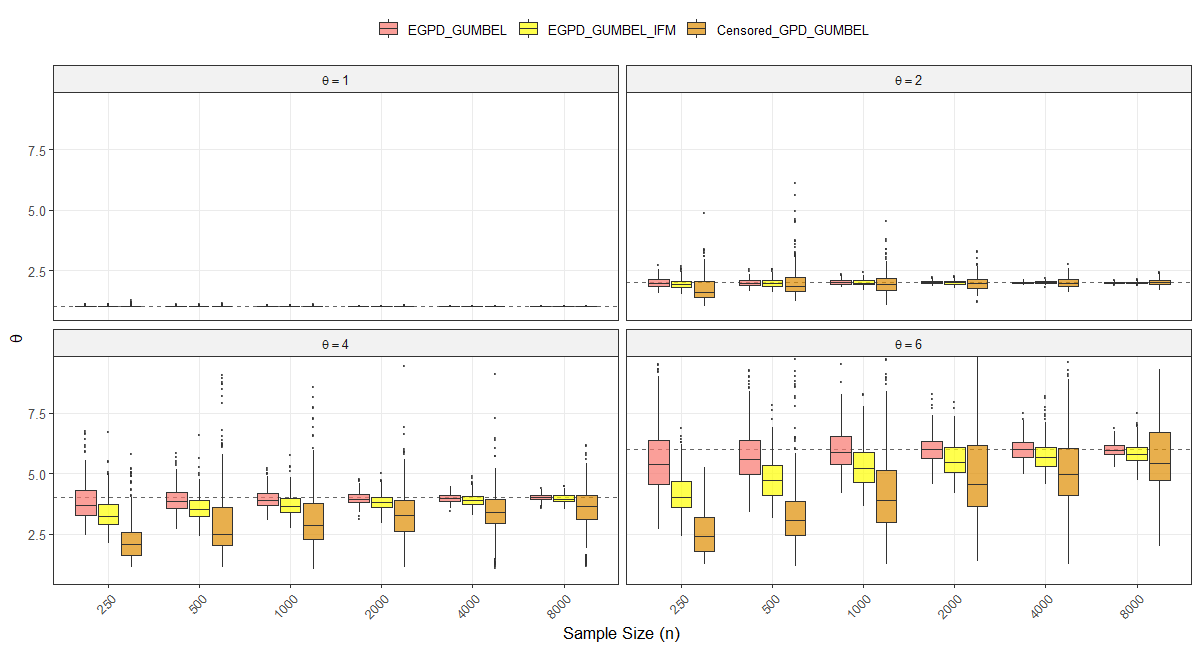
\includegraphics[width=\textwidth]{figures/sim_consistency3.png}
    \end{figure}
\end{frame}

\begin{frame}{Hill Estimates: RMSE (n = 2000)}
    \begin{figure}
        \centering
        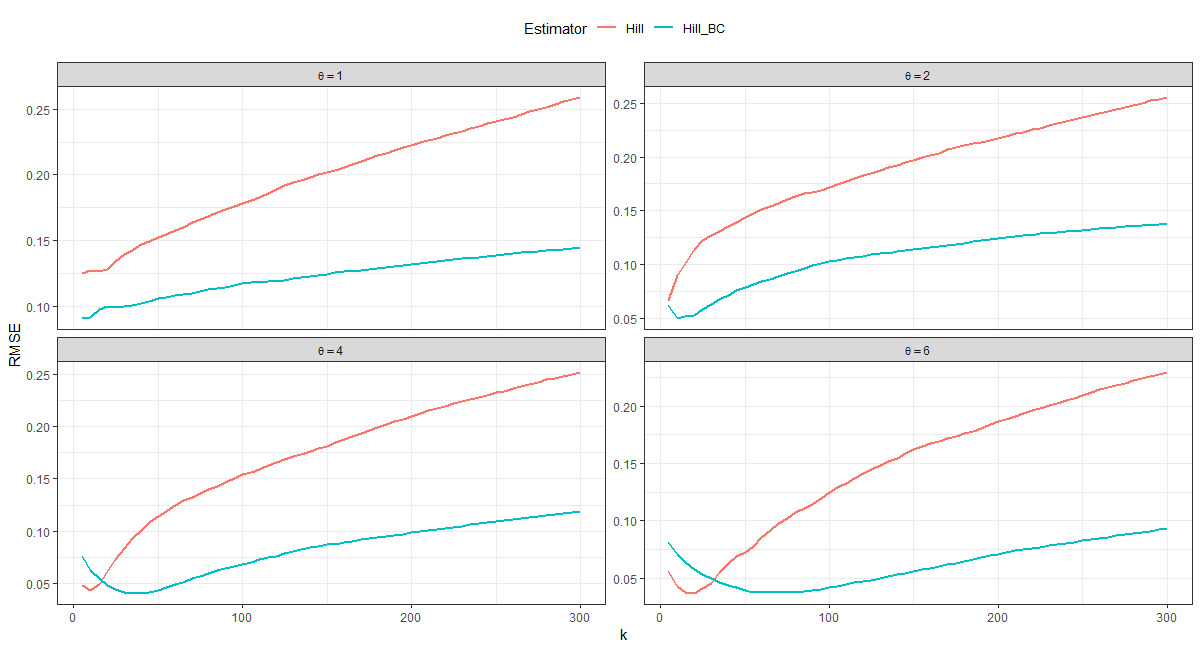
\includegraphics[width=\textwidth]{figures/hill_rmse.png}
    \end{figure}
\end{frame}

\begin{frame}{Hill Estimates: Absolute Relative Bias (n = 2000)}
    \begin{figure}
        \centering
        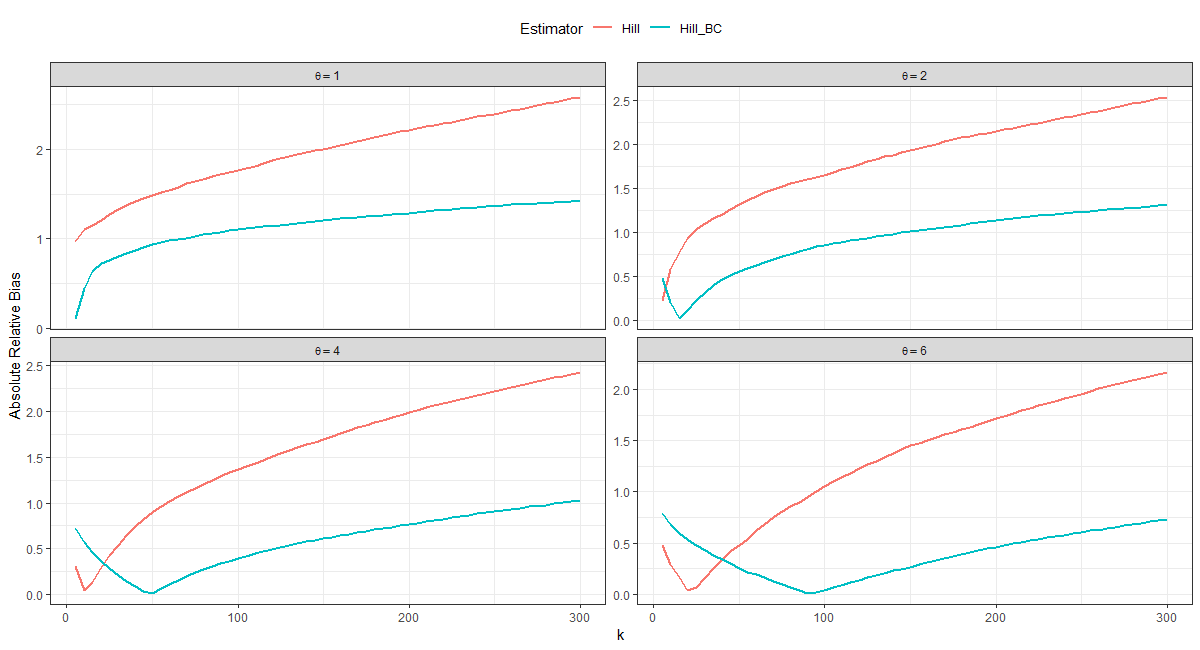
\includegraphics[width=\textwidth]{figures/hill_relbias.png}
    \end{figure}
\end{frame}

% ==========================================
% ROADMAP
% ==========================================
\section{Conclusion}

\begin{frame}{Future Directions}
\end{frame}


\begin{frame}[allowframebreaks]{References}
  \footnotesize

  \bibliographystyle{apalike} 
  
  \bibliography{ref} 
\end{frame}

\end{document}